\subsection{Custo dos gaps vistos pelos robôs do time}
Somente o peso do dos gaps vistos pelos robôs do time
alterado para zero. Os resultados no planejamento são
apresentados na figura~\ref{fig:block_goal_0}.

\begin{figure}[H]
  \centering
  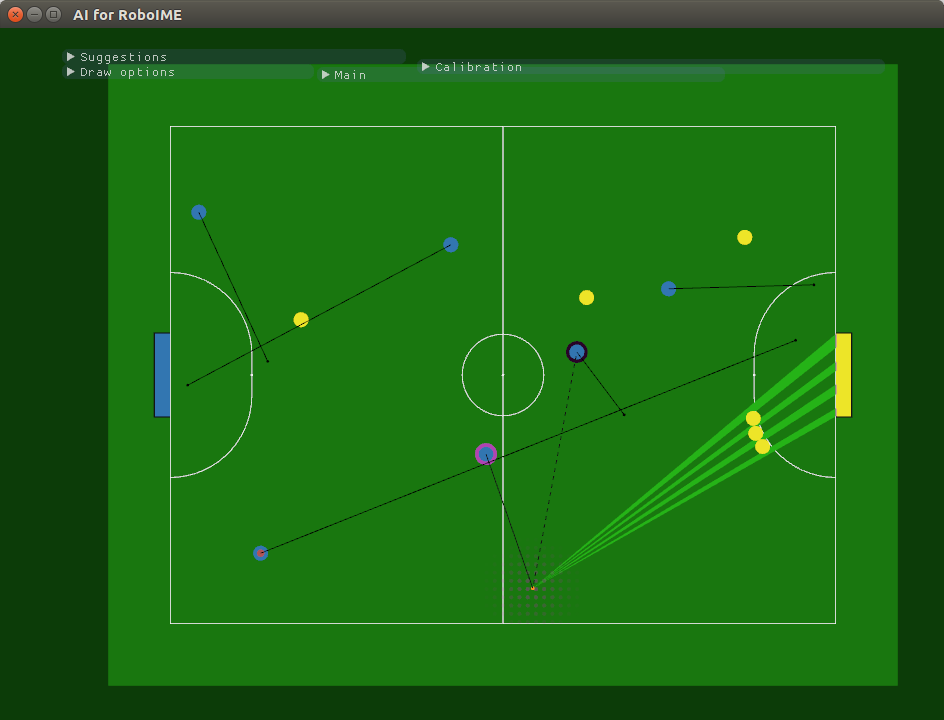
\includegraphics[width= 0.8\linewidth]{result/block_goal_atq_0}
  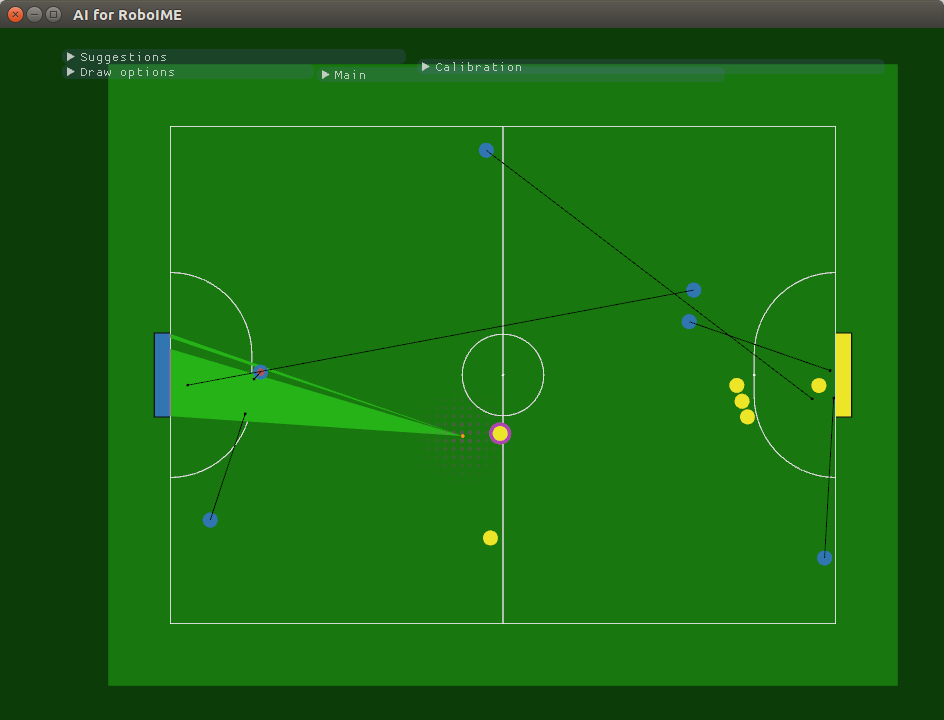
\includegraphics[width= 0.8\linewidth]{result/block_goal_def_0}
  \caption{Planejamento com os parâmetros iniciais e com o custo
           dos gaps vistos pelos robôs do time nulo.
           No ataque (acima) e na defesa (abaixo)}\label{fig:block_goal_0}
\end{figure}
